% Chapter 1

\chapter{Introduction} % Main chapter title

\label{Chapter1} % For referencing the chapter elsewhere, use \ref{Chapter1}

\lhead{Chapter 1. \emph{Introduction}} % This is for the header on each page - perhaps a shortened title

%----------------------------------------------------------------------------------------

TR-069 (Technical Report 069) is a technical specification published by the Broadband Forum and entitled CPE WAN Management Protocol (CWMP)\citep{Reference1}. It defines an application layer protocol for remote management of end-user devices. As a bidirectional SOAP/HTTP-based protocol, it provides the communication between customer-premises equipment (CPE) and Auto Configuration Servers (ACS). It includes both a safe auto configuration and the control of other CPE management functions within an integrated framework. The protocol addresses the growing number of different Internet access devices such as modems, routers, gateways, as well as end-user devices which connect to the Internet, such as set-top boxes, and VoIP-phones. The TR-069 standard was developed for automatic configuration and management of these devices by Auto Configuration Servers (ACS). The technical specifications are managed and published by the Broadband Forum. TR-069 was first published in May 2004, with amendments in 2006, 2007, 2010, July 2011 to version 1.3.[1] and November 2013 to version 1.4 (am5) [2]

On 23 October 2014, the new Smart Home product of Orange --Homelive-- is published. Homelive is a unique solution that can link to the connected objects in the home, allowing client to manage the appliances remotely.There are a range of intelligent sensors and connected devices: weather monitors, thermostats, light switches, sound and movement detectors, and smoke detectors. They are connected using the protocol Z-Wave. For the Orange support team, managing and monitoring the devices from distance is essential to reduce the maintenance fee.

The present report describes the work I have done during my six months internship at Orange Labs. In order to reduce the maintenance fee of sending support enginner to the home of client, my mission was to evaluate the adaptation of TR-069 in the Homelive in order to manage devices using ACS from distance. The fommowing part of this chapter will at first give a basic conception of the context, I will then present the objective of my internship. At the last section, the outline of the report wil be listed.

%----------------------------------------------------------------------------------------

\section{Context}
\subsection{Smart Home}

Home automation \citep{homeautomation} is the residential extension of building automation. It is automation of the home, housework or household activity. Home automation may include centralized control of lighting, HVAC (heating, ventilation and air conditioning), appliances, security locks of gates and doors and other systems, to provide improved convenience, comfort, energy efficiency and security. Home automation for the elderly and disabled can provide increased quality of life for persons who might otherwise require caregivers or institutional care.

The popularity of home automation has been increasing greatly in recent years due to much higher affordability and simplicity through smartphone and tablet connectivity. The concept of the "Internet of Things" has tied in closely with the popularization of home automation.

A home automation system \citep{homeautomation1} integrates electrical devices in a house with each other. The techniques employed in home automation include those in building automation as well as the control of domestic activities, such as home entertainment systems, houseplant and yard watering, pet feeding, changing the ambiance "scenes" for different events (such as dinners or parties), lighting control system, and the use of domestic robots. Devices may be connected through a home network to allow control by a personal computer, and may allow remote access from the internet. Through the integration of information technologies with the home environment, systems and appliances can communicate in an integrated manner which results in convenience, energy efficiency, and safety benefits.

Orange contribution in standards aims at preparing an enhanced experience for the end-user, with a simplified approach in terms of in-home connectivity of the devices. It also targets an interoperable infrastructure, through a reference smart home architecture attracting various application providers, because the variety of relevant applications is a key element for the smart home market to take-off. This implies the availability of unified, open APIs proposed to the developers that do not want to deeply study each specific way to access the functionalities from all possible underlying technologies. Harmonization of data models is also a key standardization objective for Orange to propose smart home services in a seamless and progressive way to the end-user.
%------------------------------------------------------------------------------------------------------------------------------------------------------------
\subsection{Homelive Offer}

Homelive is a smart-home convenience system that puts their home at the customer’s fingertips when away. Using a single application accessed by a smartphone tablet or computer, Orange Homelive allows consumers to adjust settings and to control remotely all connected home appliances from any place in order to enhance home security, improve home comfort, and manage energy consumption in the home. Homelive includes support for a broad range of devices, and Orange is continuing to expand the types of services and devices supported. The home monitoring subscription service is available for 9.99EUR per month, and sends alerts when devices such as motion detectors and smoke alarms are triggered to owners via SMS or email.

The Homelive pack is sold for 79 euros (\$99.00) with a special cash back offer of 78 euros — offer is valid for all new Homelive customers. It includes a central unit and 3 devices — a smoke sensor, a door/window sensor and a motion sensor(\fref{fig:1}). To enjoy the features of the Homelive solution, the user pays only 9.99 euros per month with a 12-month commitment. The subscription includes unlimited SMS alerts, continuity of service monitoring and alerts in case of internet failure (subject to Orange mobile coverage), dedicated technical support and storage of video and data for a month. The offer is not restricted to Orange customers. Homelive can be installed in any home in France with an active Internet connection(\fref{fig:2}).

\begin{figure}[htbp]
	\centering
		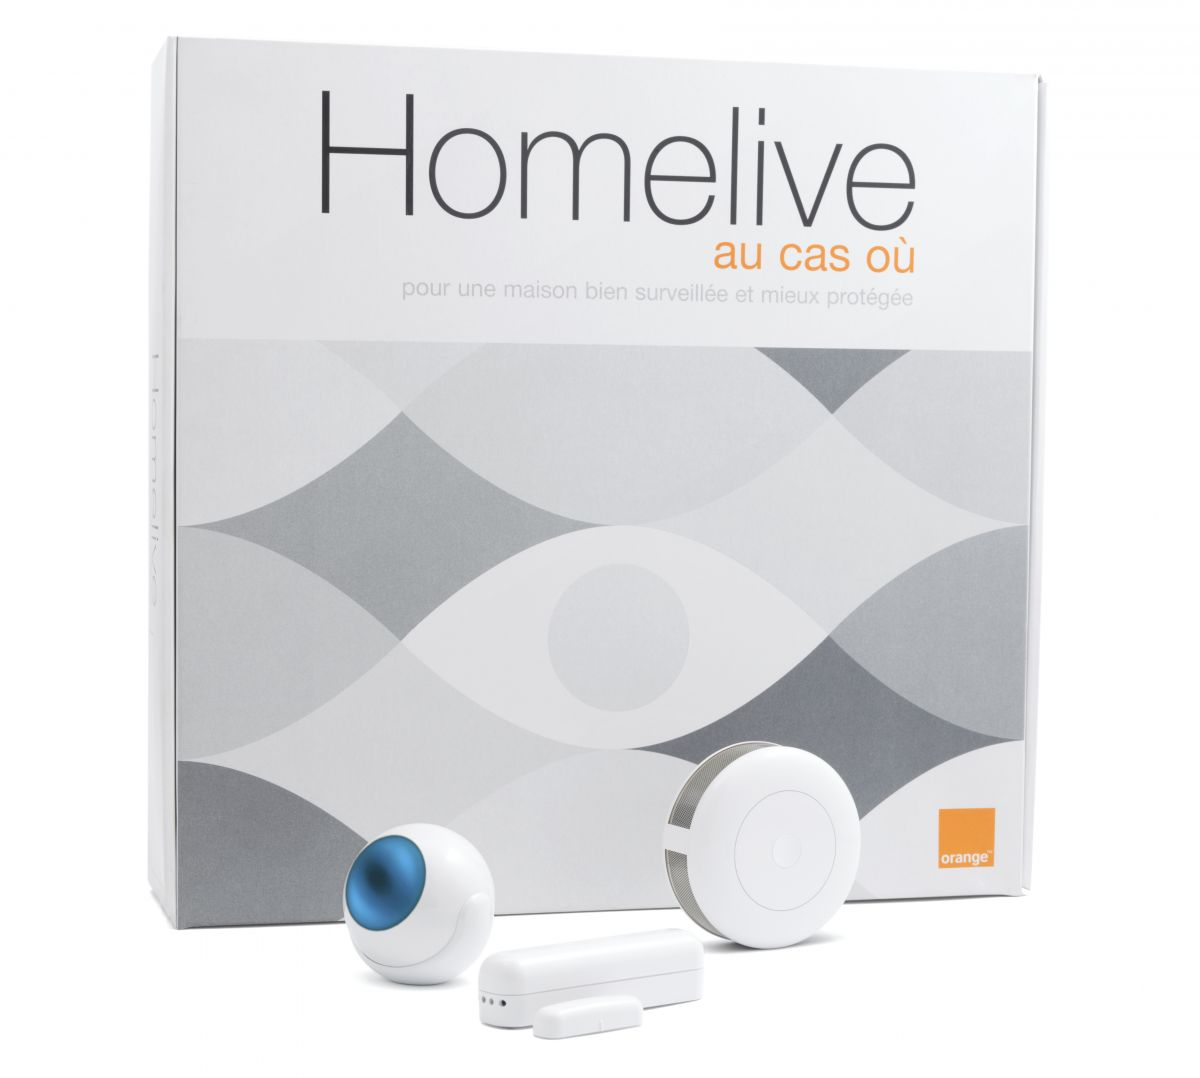
\includegraphics[width=10cm]{Figures/Pack_Accesoires_Homelive.jpg}
	\caption[Homelive Offre Au Cas Où]{Homelive Offre Au Cas Où.}%{}
	\label{fig:1}
\end{figure}

\begin{figure}[htbp]
	\centering
		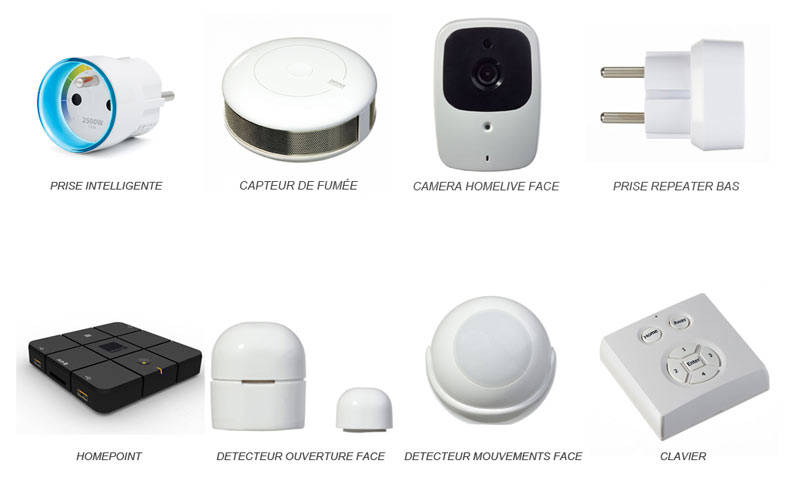
\includegraphics[width=10cm]{Figures/home-live_capteurs.jpg}
	\caption[Homelive Sensors]{Homelive Sensors.}%{}
	\label{fig:2}
\end{figure}
%------------------------------------------------------------------------------
\subsection{Device Management}
The home networking is becoming a reality : a growing number of devices are connected in the user's home network and require device management. Device management is a key asset for Orange used to upgrade the livebox or Homelive firmware for new services deployment; it also used for VoIP activation and next generation liveradio & IPTV set-top box. Orange is operating a TR69 platform called Karma.

Service providers are faced with the new challenge of \textbf{managing the increasing complexity} of the home devices. Home Device Management addresses the technical device management and includes the following operations:
%------------------------------------------------------------------------------
\begin{itemize}
  \it
  \setstretch{1} % Reset the line-spacing to 1
  \item Setup and configuration of services (auto-provisioning).
  \item Managing connected devices (local or remote management): basic management, configuration management, software management, performance monitoring.
  \item Giving Service Providers more control (firmware upgrade).
	\item Cost reduction through remote management (avoid problem).
\end{itemize}
%------------------------------------------------------------------------------
Concerning the management of the connected devices, management could mainly be defined as follow:
\begin{itemize}
  \it
  \setstretch{1} % Reset the line-spacing to 1
  \item \textbf{Basic Management :} Enable reboot, baseline reset, logging and basic test features such as ping, traceroute, nslookup and self-test action.
  \item \textbf{Configuration Management :} Includes Data Model access and setting, i.e., parameter setting and object creation.
  \item \textbf{Software Management :} Enable Deployment Unit, i.e., installation/uninstallation/update of software package; Execution Unit, i.e., active unit, start and stop.
	\item \textbf{Performance Monitoring :} Include time base mechanism to retrieve information on the device behavior, i.e., raw, threshold or aggregated.
\end{itemize}
%------------------------------------------------------------------------------
Software vendors proposes several solutions to achieve these goals based on proprietary or standardized protocols. There are several standardization initiatives but the Broadband Forum Home is the more interested proposal to address remote Home Device Management needs from the operator point of view.

The core protocol CWMP (CPE Wan Management Protocol, also known as TR-069) is developped in the Broadband Forum. The data models are produced by the Broadband Forum based on other organisation input. The data model leaves quite a lot of options. Standard organisation or forum like HGI or ETSI TISPAN proposes implementation profiles requiring certain paramaters as mandatory.

Nevertheless, TR-069 is not well adopted by manufacturers, especially consumer electronic vendors. To achieve local Home Device Management the UPnP Forum has created a Working Committee dedicated to Device Management namely: \textbf{UPnP Device Management}. Orange is currently co-chairing it with Samsung. This working committee is defining a local management protocol which is able to cover the remote management scope, i.e., from a local/inner point of view, and to manipulate Data Model definitions coming from other fora such as Brodband Forum or OMA.
%------------------------------------

During these six months, I integrated in the I23 group and focused on scientific computing and its optimization with computational accelerators. The group has about 20 members. Generally speaking, they have a formal meeting every two weeks (réunion du groupe). Small technique gatherings are more frequent among the people in the same project. Communication for group members is convenient since all offices are closed. Moreover, EDF provides staff members with internal message and telephone service, which improve working efficiency as well.
%----------------------------------------------------------------------------------------

\section{Outline}
A very initial investigation on the ray tracing CPU/GPU portability of MODERATO will be introduced in this report. In a first part I will introduce the radiographic inspection and its simulation with MODERATO. Then I will briefly give some details on several popular HPC (High Performance Computing) accelerators: CPU cluster, Xeon Phi and GPGPU. At the end of this part, two available ray tracing framework for scientific calculations will be described.

Chapter 3 will cover how to build ray tracing softwares with OptiX framework. It first explains programming models defined in OptiX. OptiX \textit{Host Objects} and \textit{Device Programs} will be detailed with code examples. Besides, how to perform CUDA/OptiX communications and the comparison of three RNGs (Random Number Generators) will be presented. At last, OptiX performance guidelines and programming caveats help a more efficient implementation work.

The following chapter focuses on modeling process in OptiX. The procedure of porting the original code to OptiX will be described. Then, it goes over several important points of our OptiX implementation. Optimizations like reductions and selection of RNGs will be discussed. Problems and corresponding solutions will be fully detailed at the end of this chapter.

The final chapter introduces the tests we have done to evaluate and validate the OptiX implementation. Firstly, test configurations such as models of sources, inspected objects and detectors will be presented. Then, in order to verify effectiveness and accuracy of CUDA Fast-Math Intrinsic Functions (Compared to the traditional IEEE 754 standard), tests on this item will be presented with explanations. Moreover, kernel size can have an influence on ray tracing performance as well: even if a 1000$\times$1000 kernel has been proved to be more productive than a 500$\times$500 one on calculations, its poor efficiency during initialization may always be a non-negligible drawback. Therefore, some tests were realized to find the optimal balance between calculation and initialization. Another test concerns the degradation of serialized operations during parallel computing: utilization of atomic operations within OptiX and their accuracy will be discussed. The chapter also evaluates OptiX performance by comparing it with a CPU cluster. In the end, the chapter draws conclusions from the previous test results. Apart from the advantages on using OptiX, difficulties and inconveniences during implementation will be discussed. After these concluding remarks, a future road-map for this OptiX implementation is proposed, and the amount of work needed to make it featured.
